% !TEX TS-program = pdflatex
% !TEX encoding = UTF-8 Unicode

% This is a simple template for a LaTeX document using the "article" class.
% See "book", "report", "letter" for other types of document.

\documentclass[11pt]{article} % use larger type; default would be 10pt

\usepackage[utf8]{inputenc} % set input encoding (not needed with XeLaTeX)

%%% Examples of Article customizations
% These packages are optional, depending whether you want the features they provide.
% See the LaTeX Companion or other references for full information.

%%% PAGE DIMENSIONS
\newcommand{\br}{\mathbf{r}}
\newcommand{\bM}{\mathbf{M}}
\newcommand{\cK}{\mathcal{K}}
\usepackage{graphicx} % support the \includegraphics command and options

% \usepackage[parfill]{parskip} % Activate to begin paragraphs with an empty line rather than an indent

%%% PACKAGES
\usepackage{booktabs} % for much better looking tables
\usepackage{array} % for better arrays (eg matrices) in maths
\usepackage{paralist} % very flexible & customisable lists (eg. enumerate/itemize, etc.)
\usepackage{verbatim} % adds environment for commenting out blocks of text & for better verbatim
\usepackage{subfig} % make it possible to include more than one captioned figure/table in a single float
% These packages are all incorporated in the memoir class to one degree or another...
\usepackage{tikz-cd}
\usepackage{circuitikz}
%\usepackage{wasysym}
\usepackage{ textcomp }
\usepackage{macros}

%%% HEADERS & FOOTERS
\usepackage{fancyhdr} % This should be set AFTER setting up the page geometry
\pagestyle{fancy} % options: empty , plain , fancy
\renewcommand{\headrulewidth}{0pt} % customise the layout...
\lhead{}\chead{}\rhead{}
\lfoot{}\cfoot{\thepage}\rfoot{}

%%% SECTION TITLE APPEARANCE
%\usepackage{sectsty}
%\allsectionsfont{\sffamily\mdseries\upshape} % (See the fntguide.pdf for font help)
% (This matches ConTeXt defaults)

%%% ToC (table of contents) APPEARANCE
\usepackage[affil-it]{authblk}
\usepackage[nottoc,notlof,notlot]{tocbibind} % Put the bibliography in the ToC
\usepackage[titles,subfigure]{tocloft} % Alter the style of the Table of Contents
\renewcommand{\cftsecfont}{\rmfamily\mdseries\upshape}
\renewcommand{\cftsecpagefont}{\rmfamily\mdseries\upshape} % No bold!

\newcommand{\NTT}{{\bf NTT }}
\newcommand{\INTT}{{\bf INTT }}
\newcommand{\MM}{{\bf MM }}
\newcommand{\M}{{\bf M}}
\newcommand{\NUSS}{{\bf NUSS }}
\newcommand{\Enc}{{\bf Enc }}
\newcommand{\Relin}{{\bf Relin }}
%%% END Article customizations

\usepackage{amsthm}
\theoremstyle{plain}
\newtheorem{theorem}{Theorem}
\newtheorem{claim}{Claim}
\newtheorem{fact}{Fact}

\theoremstyle{definition}
\newtheorem{definition}{Definition}
\def\rem#1{{\marginpar{\raggedright\scriptsize #1}}}

%%% The "real" document content comes below...

\title{Optimizing relinearization in circuits for homomorphic encryption}

\author[]{Hao Chen}
\affil{\small{Microsoft Research, Redmond WA, USA} \\

\texttt{haoche@microsoft.com}}
\date{}
\begin{document}
\maketitle  % Activate to display a given date or no date (if empty),
         % otherwise the current date is printed 


\begin{abstract}
Fully homomorphic encryption (FHE) allows an untrusted party to evaluate arithmetic circuits,  i.e., perform additions and multiplications on encrypted data, without having the decryption key. 


Currently, the most widely known FHE schemes are those based on the hardness of the RLWE problem, and they share some common features. Ciphertext sizes grow after each homomorphic multiplication; multiplication is much more costly than addition, and the cost of homomorphic multiplication scales linearly with the input ciphertext sizes. Furthermore, there is a special {\it relinearization} operation that reduce the size of a ciphertext, and the cost of relinearization is on the same order of magnitude as homomorpic multiplication. This motivates us to define a discrete optimization problem, which is to decide where (and how much) in a given circuit to relinearize,  in order to minimize the total computational cost. 

In this paper, we formally define the {\it relinearize problem}. We prove that the problem is NP-hard. In addition, in the special case where each vertex has at most one outgoing edge, we give a polynomial-time algorithm. 
\end{abstract}

\section{Introduction}

Fully homomorphic encryption (FHE) is an encryption technique which allows any untrusted party to evaluate functions on encrypted data.  As a typical application, FHE allows a client to outsource computation to an untrusted cloud. It has generated great interest in fields such as health and finance, due to the need to analyze sensitive data without having access to the data itself. Since Gentry introduced the first FHE scheme in 2009, there has been a line of works that proposed new FHE schemes with improved efficiency, among which two of the most widely used schemes are \cite{brakerski2014leveled} and its scale-invariant counterpart \cite{fan2012somewhat}. Implementations of these schemes include \cite{halevi2014algorithms}, \cite{chensimple}, and \cite{aguilar2016nfllib}. There has been numerous work that design applications based on these schemes. Some of them (\cite{gilad2016cryptonets,bos2017privacy}) evaluate machine learning models on encrypted data. Others use FHE to design secure protocols such as private information retrieval \cite{melchor2016xpir} and private set intersection \cite{chen2017fast}.



Unfortunately, in these schemes homomorphic operations are still several-orders of magnitude slower than performing the same operation on plaintexts. Therefore, any optimization in the computation time has great interest.

In order to use FHE to evaluate a function, one first needs to express the function as an arithmetic circuit. The circuit is represented as a direct acyclic graph with each vertex being either an input, a multiplication, or an addition. In both schemes mentioned above, a fresh ciphertext is a vector of length two. When a homomorphic multiplication is performed, the length of the output ciphertext grows. More precisely, if we denote the 
length of a ciphertext $c$ by $l(c)$, then $l(  c_1 \otimes c_2 ) = l(c_1) +  l(c_2) - 1$. The length of the result of a homomorphic addition is the maximum length of the two operands, i.e., $l(  c_1 \oplus c_2 ) = \max\{l(c_1), l(c_2)\}$. 

Rouhgly speaking, the computational cost to perform a homomorphic multiplication scales linearly with its input lengths. In both schemes, 
we can model the amount of work it takes to perform a homomorphic multiplication between two ciphertexts $c_1$ and $c_2$ by 
\[
	k_m (l(c_1) + l(c_2)), 
\] 
where $k_m$ is some scheme-dependent constant. In FHE, there is also a squaring operation, which takes as input an encryption of $x$ and returns an encryption of $x^2$. It has the same cost and length effect as multiplication, but only takes one input. 


Homomorphic additions, on the other hand, takes much less time to perform compared to multiplication. Hence in this work we will assume that additions are ``free''.  For the same reason, we will adopt the common notation from the FHE literature, and denote by depth of a circuit by the largest number of multiplication vertices contained in a path. 

Note that it is undesirable to let the ciphertext sizes grow, since it will increase both the computational cost and the storage burden. To control the ciphertext sizes, both schemes support a special operation called \emph{Relinearization}. Effectively, relinearizing a ciphertext means reducing its length, while keeping the underlying message the same. We can use this operation to reduce the length of a ciphertext to any integer between two and its original length.  The cost of relinearization scales linearly with the reduction in ciphertext length. In other words, there exists a constant $k_r$ such that reducing the ciphertext lengths by $i$ takes $i \cdot k_r $ units of work. 

Suppose we are given an arithmetic circuit to perform on encrypted inputs. It is now an optimization problem to decide where and how much to relinearize, in order to minimize the total amount of work, consisting of multiplication cost and relinearization cost. Previous works almost always employ a simple strategy, which is to relinearize at every multiplication. In this way, the multiplication costs are kept minimal, since the lengths of inputs to any multiplication vertex are always 2 -- the smallest possible. 

In Section 2, we will formally describe the problem and show why this simple strategy can be sub-optimal. In Section 3, we prove that the relinearize problem is NP-hard by reducing from the knapsack problem. Finally, in Section 4, we restrict to the special case where each vertex in the circuit has at most one outgoing edge, and give a polynomial time algorithm. 

\subsection{Related work}

The work \cite{carpov2015armadillo} is an effort to 
find a good circuit representation of a function, in order to minimize the total computation time. 

Bootstrapping is an operation that refreshes the so-called noise in FHE ciphertexts. It is an essential yet expensive operation. The two papers \cite{lepoint2013minimal} and \cite{benhamouda2017optimization} aim at minimizing the total number of bootstrapping operations in a circuit, while keeping the noise from overflowing in order to ensure the final result is correct. In their work, the authors implicitly assume the relinearization is done after every multiplication. Similarly, we will make a simplifying assumption that the boostrapping time is a constant, so that it does not factor into our optimizatoin problem. It will be interesting to combine these works in order to achieve an overall optimization that targets both operations. 


{\bf Acknowledgement} The author thanks Rebecca Hoberg and Mohit Singh for helpful discussions in preparing this work. 



\section{Problem Description}

To formally describe our problem, we need to properly define circuits used in FHE applications. 

\begin{definition}
a (squaring-enabled) arithmetic circuit is a directed acyclic graph $G = (V,E)$, where there are three kinds of vertices: input vertices has indegree 0 and outdegree 1; output vertices has indegree $\in \{1, 2\}$ and outdegree 0; add/multiply operation vertices have indegree 2 and outdegree 1; finally, square operation vertices have indegree and outdegree both equal to 1. 
\end{definition}

We will define the relinearize problem as an integer programming problem on  arithmetic circuits. For every vertex $i$ we maintain an integer variable $l^{new}(i)$ (the final length of vertex $i$ during homomorphic evaluation of $G$), and an integer 
variable $x_i$, which indicates the amount of relinearization at $i$. We will denote the two parents of a vertex $i$ by $p_1(i)$ and $p_2(i)$. By convention, if $i$ is a squaring node, then we set $p_1(i) = p_2(i)$. We denote addition vertices by $\oplus$ and multiplication/square vertices by $\otimes$. To resolve ambiguity, we make the convention that if a $\otimes$ vertex has two distinct parents, then it is understood as a multiplication; otherwise it is a squaring.

Then the {\it relinearize problem} on $G$ is 
\[
	\mbox{minimize } k_r \sum_{i \in V } x_i  + \sum_{i = \otimes} k_m (l^{new}(i) + x_i), 
\]
s.t. 

\begin{align*}
l^{new}(i) \geq 2  & \qquad &\mbox{ for all } i \\ 
l^{new}(i)  = l^{new}(p_1(i)) + l^{new}(p_2(i)) - 1 - x_i  & \qquad & \mbox{if } i = \otimes \\ 
l^{new}(i)  \geq l^{new}(p_1(i))  - x_i  & \qquad & \mbox{if } i = \oplus \\ 
l^{new}(i)  \geq l^{new}(p_2(i))  - x_i  & \qquad & \mbox{if } i = \oplus \\
x_i, l^{new}(i) \in \bZ_{\geq 0}  & \qquad &\mbox{ for all } i \\
\end{align*}

\subsection{An example} To demonstrate the non-trivality of the relinearize problem,  we consider the following circuit: 
\begin{center}
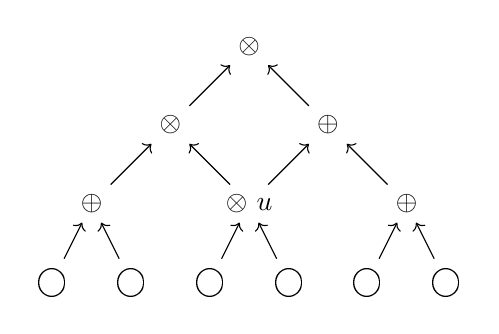
\begin{tikzpicture}[commutative diagrams/every diagram] 
\node (Pfinal) at (2,2) {$\otimes$}; 
\node (P1) at (1,1) {$\otimes$} ; 
\node (P2) at (3,1) {$\oplus$};
\node (P3) at (0,0) {$\oplus$};
\node (P4) at (2,0) {$\otimes$ $u$};
\node (P5) at (4,0) {$\oplus$};
\node (P6) at (-0.5,-1) {\textbigcircle};
\node (P7) at (0.5,-1) {\textbigcircle};
\node (P8) at (1.5,-1) {\textbigcircle};
\node (P9) at (2.5,-1) {\textbigcircle};
\node (P10) at (3.5,-1) {\textbigcircle};
\node (P11) at (4.5,-1) {\textbigcircle};
\path[commutative diagrams/.cd, every arrow, every label] 


(P1) edge node[swap] {} (Pfinal)  
(P2) edge node[swap] {} (Pfinal) 
(P3) edge (P1) 
(P4) edge (P1) 
(P4) edge node {} (P2) 
(P5) edge node {} (P2)
(P6) edge node {} (P3)
(P7) edge node[swap] {} (P3)
(P8) edge node {} (P4)
(P9) edge node[swap] {} (P4)
(P10) edge node  {}  (P5)
(P11) edge node[swap] {} (P5);
\end{tikzpicture}
\end{center}

First, we apply the simple strategy and relinearize at every multiplication vertex. Then the total cost is equal to $12 k_m + 3k_r$. 

%The costs and lengths of the nodes are labeled as below: (we have used \red{red} for length and \blue{ blue} for multiplication cost, green for relinearization cost ). 

\iffalse
\begin{center}
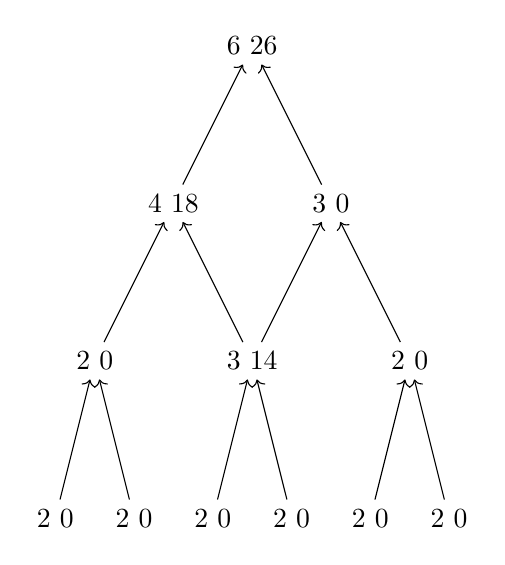
\begin{tikzpicture}[commutative diagrams/every diagram] 
\node (P0) at (2,5) {\red{6} \blue{26}}; 
\node (P1) at (1,3) {\red{4} \blue{18}} ; 
\node (P2) at (3,3) {\red{3} \blue{0}};
\node (P3) at (0,1) {\red{2} \blue{0}};
\node (P4) at (2,1) {\red{3} \blue{14}};
\node (P5) at (4,1) {\red{2} \blue{0}};
\node (P6) at (-0.5,-1) {\red{2} \blue{0}};
\node (P7) at (0.5,-1) {\red{2} \blue{0}};
\node (P8) at (1.5,-1) {\red{2} \blue{0}};
\node (P9) at (2.5,-1) {\red{2} \blue{0}};
\node (P10) at (3.5,-1) {\red{2} \blue{0}};
\node (P11) at (4.5,-1) {\red{2} \blue{0}};
\path[commutative diagrams/.cd, every arrow, every label] 

(P1) edge node[swap] {} (P0)  
(P2) edge node[swap] {} (P0) 
(P3) edge node {} (P1) 
(P4) edge node {} (P1) 
(P4) edge node {} (P2) 
(P5) edge node {} (P2)
(P6) edge node {} (P3)
(P7) edge node[swap] {} (P3)
(P8) edge node {} (P4)
(P9) edge node[swap] {} (P4)
(P10) edge node  {}  (P5)
(P11) edge node[swap] {} (P5);
\end{tikzpicture}
\end{center}
The total cost is 14 + 18 + 26 = 58.  (FIXME) 
\fi
Alternatively, we can choose to only relinearize the vertex $u$. Then the multiplication cost increases to $14k_m$, while the relinearization cost is $k_r$, so the total cost is $14k_m + k_r$. Comparing this with the previous cost, we see that as long as  $k_r > k_m$, the simple strategy is not optimal. 


% {\it Question}: does there exist a polynomial time algorithm for the Relinearization problem?

\iffalse
\section{Some initial ideas}

\subsection{Integer Programming approach}


%Mohit suggested that the original problem might be NP-hard. But for our input sizes maybe 
%integer programming will solve it pretty fast. 




Then we plug it into some integer programming solver to obtain an optimal result. 

Fact: the optimal solution of the above Integer programming problem always corresponds to a meaningful solution to the relinearization problem, i.e. the max is achieved at every node. Informal proof: if not, we could decrease the $x_i$ on the node by 1 and have the same effect, so the objective function is even smaller

As an example, we consider the following simple circuit. 
\begin{center}
\begin{tikzpicture}[commutative diagrams/every diagram] 
\node (P0) at (2,6) {Dec}; 
\node (Pfinal) at (2,5) {$\otimes$}; 
\node (P1) at (1,3) {$\otimes$} ; 
\node (P2) at (3,3) {$\oplus$};
\node (P3) at (0,1) {$I$};
\node (P4) at (2,1) {$I$};
\node (P5) at (4,1) {$I$};
\path[commutative diagrams/.cd, every arrow, every label] 


(Pfinal) edge node[swap] {} (P0) 
(P1) edge node[swap] {} (Pfinal)  
(P2) edge node[swap] {} (Pfinal) 
(P3) edge node {} (P1) 
(P4) edge node {} (P1) 
(P4) edge node {} (P2) 
(P5) edge node {} (P2); 
\end{tikzpicture}
\end{center}

We label the nodes from top-down, left-right so that Dec is the 0-th node. Then the objective function 
can be writeen as 
\[
	k(x_0 + x_1 + x_2 + x_3 )  - 4( l^{old}(1) - l^{new}(1) )  -  4( l^{old}(2) - l^{new}(2) )  -  l^{old}(0) + l^{new}(0). 
\]	
The constraints are:  \\
\[
\begin{cases}
l^{new}(i) \geq 2,  i  = 0,1,2,3.  \\
l^{new}(1) = l^{new}(2) + l^{new}(3) -1 - x_1 \\
l^{new}(2) = l^{new}(4) + l^{new}(5) -1 - x_2 \\
l^{new}(3) \geq l^{new}(5) - x_3 \\ 
l^{new}(3) \geq l^{new}(6) - x_3 \\
x_i \geq 0. 
\end{cases}
\]
%New observation: the old lengths are not needed at all! All we need to know is that the input lengths 
%are fixed.  (This makes sense because the lengths are computed from input lengths). 

\subsection{Submodularity and the binary relinearization problem}

Given an arithmetic circuit defined in previous sections, the cost function $F(x_1, \ldots, x_n)$, where the $x_i$ are positive integers indicating the amount of Relinearization done at the $i$-th node. Now if we only allow relinearization to reduce the size of ciphertexts by at most 1, i.e., $x_i \in \{0, 1\}$ for all $i$, then the problem is called \emph{binary relinearization problem}. In this case, I think cost function should be submodular, and thus there is a polynomial time algorithm to minimize the cost. More precisely, define a set function 
\[
	G: 2^{[n]} \to \bR: G(S) = F(\sum_{i \in S}e_i). 
\]
For example, $G(\{1,2,3\}) = F(e_1 + e_2 + e_3)$.  

\begin{lemma}
$G$ is submodular. 
\end{lemma}
Proof: intuitively, the total cost of doing relin diminishes when the environment is ``shorter''. 

\begin{corollary}
the binary relinearization problem can be solved in polynomial time. 
\end{corollary}

Some new ideas: 

Lemma: for each $i$ we have ``diminishing returns'', i.e.,  $|F(v + 2e_i) - F(v) |  \leq 2 |F(v+e_i) - F(v)|$. 

Proof: we can prove this inductively. First we replace $F$  with $F_0$ which gets rid of relin cost. Since relin cost is linear this does not change the inequality. Suppose the edges out of vertex $i$ are $j_1, \ldots ,j_K$. We can inductively prove an inequality in change of length. 
\[
	\Delta(length(j, 2)) \leq 2\Delta(length(j,1)), \forall j.  
\]


First, if there is no $i \to j$ path, then both sides are zero. Trivially true. 

If the level of $j$ is one more than level of $i$ and $(i,j)$ is an edge, then it's true (equality holds when 
$j$ is a multiplication node or decryption node, strict inequality can happen if $j$ is an addition). This proves the base case when $L(j) = L(i) + 1$. 

Now we proceed by induction: suppose $k$ is a vertex with $L(k) > L(i) + 1$. Assume the result 
holds for level $L(k) - 1$. Now there are several cases: if $k$ is a $\otimes$ node, then 


$\Delta(l(k, 2))  = \Delta(l(c_1(k), 2)) + \Delta(l(c_2(k), 2)) \leq 2(\Delta(l(c_1(k), 1)) + \Delta(l(c_2(k), 1))) = \Delta(l(k,1))$. 

If $k$ is an $\oplus$, suppose the lengths of childs without change is $l(c_1(k)) = x$ and $l(c_2(k)) = y$.
WLOG $x \geq y$, so $l(k) = x$. Now we can utilize a simple inequality 
\[
	| \max \{ x-a, y - b\} - \max \{x, y\} |  \leq \max \{a, b\}. \forall a,b \geq 0. 
\]
Using this inequality in our scenario, let $a = \Delta(l(c_1(k), 1) and b = \Delta(l(c_2(k), 1)$. We 
deal with each case separately. 

(1): if $x - a \leq y -b$, then $\Delta(l(k,1)) = x - y + b$. We also have $\Delta(l(k,2)) \leq x - (y - b')$. 
Combining with $b' \leq 2b$ and $x - y \geq 0$ gives the result.

(2): if $x-a > y-b$, then $\Delta(l(k,1)) = a$, and we have $\Delta(l(k,2)) \leq x - (x-a') = a'$. The result
follows from $a' \leq 2a$. 


Finally, if $k$ is Decryption node, then it is trivial. So the induction is done and we have proved that 
$$|F(v + 2e_i) - F(v) |  \leq 2 |F(v+e_i) - F(v)|.$$ for any $v \in \bZ_{\geq 0}^n$ and any $i \in [n]$ such that $v + 2e_i$ is feasible. 

Now we can prove the following crucial proposition. For an integer $v$ let $\delta(v) = 1$ if $v \neq 0$
and 0 if $v = 0$. For a vector $v$, let $\delta(v) = (\delta(v_i))_i$. 

Proposition: if $v \geq u$ and  $F(v)  > F(u)$, then $F( \delta(v-u) + u) > F(u)$. In otherwords, it suffices 
to go ``one step'' to reduce the cost. 

Proof: suppose $v_1 - u_1 \geq 2$,  applying the lemma we get 
$F(v) - F(u) \leq 2(F(v-e_1)) - F(u))$, so $F(v-e_1) > F(u)$. Keep doing this for each coordinate until we arrive at $F( \delta(v-u) + u) > F(u)$. This completes the proof. 


Now this combined with the submodular result gives the optimal choice. 


Corollary: if $u \geq 0$ is a feasible solution such that $u$ is optimal w.r.t. one-step Relin, equivalently, 
that 
\[
	F(u + \sum_{i \in S} \epsilon_i e_i) \geq F(u), \, \forall S \subseteq [n], \epsilon_i \in \{0, 1\}. 
\] 
Then $u$ is the global optimal to the Relin problem, i.e., 
\[
	F(u) = \min \{ F(v): v \mbox{ feasible } \}.  
\] 

Algorithm: keep solving forward one-step relin until optimal is reached. Proof of correctness? Polynomial 
time for sure since the total cost is integer and $O(|V|^2)$. 

Need proof: 

New: can we prove that $\Delta(a,b) \leq \frac{a+b}{2} \Delta(1,1)$?  No. But can we prove that 
$$\Delta(a,b) \leq \max(a,b) \Delta(1,1)?$$ Suppose this is Okay by induction. Then we can use induction
to prove...

\section{A proof?}

We first define $V_0$ = Inputs, and 
\[
	V_{i+1}   = \{ v \in V \backslash (V_0 \cup \cdots \cup V_i): \delta^{in}(v) \subseteq  (V_0 \cup \cdots \cup V_i) \}
\]
By definition the $V_i$ are disjoint. Also they form a cover of $V$. The number of nonempty $V_i$'s is 
bounded by the height of the graph $G$. 

Now the algorithm could work as follows: first decide the optimal strategy for $V_i$. (It is trivial 
for $V_0$ because one can't relin an input node). Then assume it's done for $V_i$, we decide 
the strategy for $V_{i+1}$. 

Lemma: when deciding $V_{i+1}$, either the nodes are trivially no Relin, or it has size 3, so we only need
to decide whether to Relin, and not worry about how much to Relin.

Proof: suppose process has been done for $V_0, \ldots, V_i$. Now for a node in $V_{i+1}$. If $v$ is 
multiplication and whose parents $(c_1(v), c_2(v)$ do not have length $(2,2)$, then trivally we should do No relin to $v$ because if so, we 
should have already Relined its two parents.  So the parents of $V$ must have length (2,2), and $v$ has 
length 3; if $v$ is addition, suppose the parent nodes of $v$ has length $x \geq y$.  So $l(v) = x$.  Now if 
$x > y$, then it does not make sense to Relin $v$ because otherwise we could have Relined the parent node with the same length. Suppose $x = y > 3$. Then the two parents $c_1(v)$ and $c_2(v)$  are in the 
``No Relin'' list. ... then what? not exactly holds ?  if $k = 4$ then okay. 

\section{Stuck point}

If we only do Yes/No relin, then because the cost function is submodular, we have a polynomial time solution. In general, I haven't figured out whether therer exists an example where $(1,2)$ is better than 
(0,0) but any relin combination of infinity norm $\leq 1$ is worse than $(0,0)$. If there exists an example,
I would say the problem is hard. Example is hard to construct? 

9/28 talked to Mohit. Still expecting the problem to be NP-hard. However the binary relin problem might be 
polynomial time solvable (assuming $x_i = 0$ or 1). 
\fi


\iffalse
\section{New directions}
Even  computing $ax^3 + bx^2 +cx +d$ is not clear. We can model plain multiplication as 
leaving the length unchanged and time taken to compute plainmult(x,a) is equal to length(x) + 1. 
Then we would like to optimize for example a single variable polynomial evaluation (assuming 
no relin is done). Question: how does one optimize among all circuits that computes the same 
result? 

\section{A related question}

Question: given a graph $G = (V,E)$, two functions $f: V \to \bR_+$ and $g: E \to \bR_+$. Given 
$k \in \bR$. Decide whether there exists a subgraph $G'$ of $G$ such that 
\[
	\frac{1}{|V'|} (\sum_{v \in V'} f(v) + \sum_{e \in E'} g(e) )  \geq k. 
\]
I think it's a hard problem in general. And it should be less difficult than the relin problem. 

Update: one can consider a more general type of problem: let $V$ be a finite set and $f: 2^V \to \bR_+$
be a function on subsets of $V$ (we can require that $f(\emptyset) = 0$). Let $k$ be some constant. 
The goal is to maximize among subsets $V'$ the following quantity
\[
	F(V') :=	\sum_{U \subseteq V'} f(U) - k|V'|. 
\]
Luckily I think $F$ is  a supermodular function. We can thus do something...

Want to have an example circuit and example $k$. 



\section{New thoughts}

1. Even the yes/no relin problem is not obvious submodular as it seems: suppose we have (2,3, +,3). 
Then Relin at the result node could make it less favorable to relin at the second operand! 

If we specify an independent subset $U$ of nodes i.e., no path goes from one node to another. Then the yes/no relin problem restricted on $U$ is submodular or not? (I think it is, but the recursive proof does not work?) 


Newer: if we have an independent subset of nodes, then yes/no relin should be submodular. Proof: one could recursively show that when the environment is smaller, reducing x to 2 will have a larger effect. 
So we can keep going and incuring independent sets? 

\subsection{10/7: web of same-length additions}

I think we can ``reduce the graph'' to that all nodes are either multiplication or additions where inputs have the same length. This is because additions with nonequal length can be reformed by a circuit transformation. 

\subsection{10/9}

Another related problem. Let $D = (V,A)$ be a directed acylic graph. A subset 
is closed if its satisfies the following condition: if all parents of v are in U, then $v$ is in $U$. The objective is 
\[
	\max_{U \subseteq V} \sum_{v \in \bar{U}} f(v)  - k |U|. 
\]


\subsection{Another related problem}

Suppose we have a circuit of addition nodes where all lengths are the same, and there are weights 
on each node. How do we choose Relin nodes $V'$ to minimize the cost? First assume all weights are 
equal. Then it is equal to (number of nodes reached) - (number of nodes initiated). Can it be maximized? 
This problem reduces to the relin problem. 



\section{NP-completeness of the relinearization problem (not completed)}

First we define an intermediate problem we call `'binary relinearization with atomic cost''. Then we show tat the $l_{max}$-MB problem from the french 
paper reduces to the intermediate problem. Informally, the binary relinearization problem decides on a subset of the nodes to relinearize, if one decide to relinearize a node, then its length is relinearized all the way down to the length of a fresh ciphertext (equal to 2 in our case). We also change the cost of each relinearization to 1 regardless of how much it reduces the ciphertext length. 

\begin{definition}
The binary relinearization problem is Relinearization problem with two modifications: (1) at each node, we have either $x_i = 0$ or $l^{new}(i) = 2$. (2) the cost function is 
\[
	\lambda \sum_{i = \otimes } (l^{old}(i) - l^{new}(i)) + \sum_{i: x_i > 0} 1.  
\]	
where $\lambda > 0$ could be any constant. 
\end{definition}

\subsection{Reduction from BP to BinaryRelin}

Given an instance $G = (V,E)$ of the $l_{max}$-MB problem, we first construct another arithmetic circuit $G' = (V',E')$ whose length growth mimicks the noise growth of $G$. Recall that in the bootstrapping problem, 
we have 
\[
	l(v) = \begin{cases} \max{l(p_1(v)), l(p_2(v))} + 1 & \mbox{ if } v = \otimes \\ 
	\max{l(p_1(v)), l(p_2(v))} & \mbox{ if } v = \oplus \\ 
	a & o.w. 
	\end{cases}
\]
Here $a$ is a constant. For convenience we set $a = 2$ (the paper set $a = 0$). 

In order to mimick this noise growth, we replace every $\otimes$ node by 
a $\oplus$ followed by an $\otimes$ with a fresh ciphertext  (see figure ). 
Now we have obtained a new graph $G'$ with $|V'| = O(|V|)$. 


\begin{tikzpicture}[commutative diagrams/every diagram] 
\node (Pfinal) at (2,5) {$\otimes$}; 
\node (P1) at (1,3) {$x$} ; 
\node (P2) at (3,3) {$y$};;
\path[commutative diagrams/.cd, every arrow, every label] 
(P1) edge node[swap] {} (Pfinal)  
(P2) edge node[swap] {} (Pfinal);
\end{tikzpicture}


\begin{tikzpicture}[commutative diagrams/every diagram] 
\node (Pfinal) at (2,5) {$\otimes$}; 
\node (P1) at (1,3) {$Input$} ; 
\node (P2) at (3,3) {$\oplus$};
\node (P3) at (2,1) {x};
\node (P4) at (4,1) {y};;
\path[commutative diagrams/.cd, every arrow, every label] 
(P1) edge node[swap] {} (Pfinal)  
(P2) edge node[swap] {} (Pfinal)
(P3) edge node[swap] {} (P2)
(P4) edge node[swap] {} (P2);
\end{tikzpicture}

Note that there is an natural embedding $V \to V'$ where in the above transform we map the addition node in $G$ to the addition node in $G'$. 
We will abuse notations and call the image $V$. 

In the next step, we add nodes and edges to $G'$ to obtain a graph $G''$. 
The graph $G''$ is constructed as follows: we fix a very short circuit $T$ whose end node has length $l_{max}$, and a circuit $S$ which evaluates 
the sum of all nodes in $V'$. Then we add up the result node of $S$ and $T$ to obtain a node $w$. Then we put a sequence of $k$ multiplications with fresh ciphertexts after w. Finally, we copy this result graph $K$ times with only the nodes in $G'$ as common nodes.  

Let $n = |V|$. 
\begin{lemma}
Suppose $\lambda  \leq \frac{1}{2(n-2)n + kn}$ and $K > \frac{n}{\lambda k}$. 
Then in the optimal solution of Binary Relin problem on $G''$, only the nodes in $V$ are relinearized. 
\end{lemma}

\begin{proof}
We may assume $l_{max} < n$ (otherwise the bootstrapping problem is trivial). Let $\mathscr{X}$  denote an optimal solution of the binary relin problem on $G''$. 

First, we show that for all $i$, we have $w_i \notin \mathscr{X}$. The reason is the benefit of relinearizing $w_i$ is bounded by $k\lambda n < 1$. 
As a consequence, we also have $s_i, t_i \notin \mathscr{X}$. Now consider the intermediate nodes in $S_i$ and $T_i$.  The benefit of relinearizing any set of $m$ nodes is bounded by $k \lambda n + \lambda (n-2) n $ (we assume $T$ has less than $n$ nodes). Now if $\lambda \ll 1/n^2$ we are good. (Relinearize nodes in $S_i$ has a benefit bounded by $k\lambda n$, a similar argument holds). Also any node in the final multiplication sequence is not in $\mathscr{X}$, since we could replace them by $w_i$ and 
the benefit is larger. 

At this point we know that $\mathscr{X} \subseteq V'$.  Now relinearizing at the extra $\otimes$ node introduced by the transform from $G$ to $G'$ is worse than relinearizing at its $\oplus$ parent. Therefore $\mathscr{X} \subseteq V$. 
\end{proof}

\begin{lemma}
An optimal solution to the binary relin problem on $G''$ is an optimal solution to the bootstrapping problem on $G$. 
\end{lemma}
\begin{proof}
First, by the above lemma, we can consider the solution $\mathscr{X} \subseteq V$. First we show that it's a feasible solution. i.e., the maximum 
length in $V$ after relinearization is done at each $i \in \mathscr{X}$ is bounded by $l_{max}$. First note that the maximal length of $V'$ is equal to that of $V$. Suppose the maximal length of nodes in $V'$ is larger than $l_{max}$. Then we can replace $\mathscr{X}$ by $V$. This would result 
in a increase in cost of $n - |\mathscr{X}| \leq n$. Since the length of each $w_i$ is reduced by at least one, the increase of benefit is at least $K \lambda k > n$. This is a contradiction, since $\mathscr{X}$ is an optimal solution to the 
binary relin problem.  

At this point we know $\mathscr{X}$ is a feasible solution to the bootstrapping problem. Suppose toward contradiction that it is not optimal, and let  $\mathscr{Y}$ be an optimal solution to the bootrapping problem. We consider $\mathscr{Y}$ as a solution to the binary relin problem on $G''$: the difference in costs is only in the graph $G'$ and the $K$ summation circuits $S_1, \ldots, S_K$. However, since $S_i$ consists entirely of addition nodes, changing node lengths does not have any impact on the cost. Therefore, the savings is entirely from the circuit $G'$, hence it is bounded by $n' (l_{max} - 2) \lambda \leq 2n^2 \lambda < 1$. Hence 
$cost(\mathscr{Y}) - cost(\mathscr{X}) < |\mathscr{Y}| - |\mathscr{X}| + 1 < 0$. This is a contradiction to the assumption  $\mathscr{X}$ is the optimal solution for $G''$. 
\end{proof}

From the above lemmas we immediately obtain
\begin{theorem}
There is a polynomial time reduction from $l_{max}$-MB to BinaryRelin with atomic cost. 
\end{theorem}

\subsection{Reduction from $l_{max} / 2$-approximate BinaryRelin to Relin}

The plan is to: given a BinaryRelin problem, transform it to a Relin problem. 
Then given a solution x to the Relin problem, we interpret that as a solution $f(x)$ of binary relin, and prove that it is with in $l_{max}/2$ of the optimal. 

\subsection{Relin is NP-hard assuming Unique Games conjecture}  

TODO: I have to revise this part. It is not clear that the proof works. Right now, I am not sure which one is better. 


We have a polynomial time reduction from approximate $l_{max}$-BP to 
approximate BinaryRelin preserving the approximation factor.  And we can reduce $l_{max}/2$ binary relin to Relin. 

Suppose we have a binary relin problem P, we can regard it as a relin problem $P'$. Suppose $x$ is an optimal solution to the relin problem. Let $x_i$ denote the amount of relinearization done at node $i$. Let $S = \{i: x_i > 0\}$. 
Then consider the solution $S_l$ for the binary relin problem. The computation cost of $(P', S_l)$ is less than that of $(P, S)$, due to the fact that nodes have smaller length.  The relin cost of $(P', S)$ is equal to $|S|$, 
whereas the relin cost of is equal to $\epsilon \sum_i x_i$, where $\epsilon$ can change.  


The web of addition can be solved in polynomial time: in fact we can write it as a linear programming problem and it turns out that its coefficient matrix is {\bf Totally Unimodular}. This shows that we can always use an LP solver to get an integer optimal. 

\fi

\section{NP-hardness of the Relinearize Problem}

In this section, we prove a polynomial reduction from the knapsack problem to the relinearize problem, which establishes that the latter problem is NP-hard.  First we recall the definition of  knapsack problem. 


\begin{definition}
Given positive integers $v_1, \ldots, v_n$, $w_1, \ldots ,w_n$, and $W$. The (0-1) knapsack problem is:
\begin{align*}
\mbox{maximize} \sum_{i=1}^{n} v_i x_i \\
\mbox{subject to } x_i \in \{0,1\}
\mbox{ and }  \sum w_i x_i \leq W. 
\end{align*}
\end{definition}




For our convenience, we make some modifications to the setting of the relinearize problem. We change the inputs lengths from two to one, and instead of $l(c1 \otimes c2) = l(c1) + l(c2)-1$, we maintain that $l(c1 \otimes c2) = l(c1) + l(c2)$.  Indeed, under this formulation  the length of every vertex is smaller by one. Hence it is equivalent to the original problem.

%\begin{lemma}
%Under this new formulation every node have $l'(c) = l(c) - 1$. 
%\end{lemma}

%\begin{proof}
%We fix a topological order of the circuit and proceed by induction. The base case is clear since we have the equality holds for the inputs. Now suppose we have a node $i$ with parents $p_1(i), p_2(i)$. Two cases, 
%if $i$ is multiplication, then $l'(i) = l'(p_1(i)) + l'(p_2(i)) + 1 = l(p_1(i)) - 2 + l(p_2(i)) - 2 + 1 = l(i) - 2$.  For addition nodes it is trivial. 
%\end{proof}

To prepare for the main theorem, we make some convenient definitions.  
\begin{definition}
A circuit is of type $\cL(k)$ if it consists of one input vertex, one output vertex, and multiplication/squaring vertices, such that if the first non-input vertex length is reduced from 2 to 1, then the length of the output vertex reduces by $k$.  
\end{definition}

Figure~\ref{fig: L7} is an example of $\cL(7)$. 
\begin{figure}[h!]
\begin{center}
\begin{tikzpicture}[commutative diagrams/every diagram]  
\node (P1) at (2,5) {$\otimes$}; 
\node (P2) at (2,4) {$\otimes$}; 
\node (P3) at (2,3) {$\otimes$}; 
\node (P4) at (2,2) {$\otimes$} ; 
\node (P5) at (2,1) {$\otimes$};
\node (P6) at (2,0) {\textbigcircle};;
\path[commutative diagrams/.cd, every arrow, every label] 
(P2) edge  (P1)  
(P3) edge  (P2) 
(P4) edge  (P3) 
%(P4) edge[bend right]   (P3)
(P4) edge[bend right]   (P1)
(P5) edge[bend left]   (P2)
(P5) edge (P4) 
%(P5) edge[bend right]  (P4)
(P6) edge (P5) 
%(P6) edge[bend right]  (P5);
%(P1) edge node {} (P0)  
%(P2) edge node[bend left] {} (P1)
%(P3) edge node[swap] {} (P2);
\end{tikzpicture}
\end{center}
\caption{an example of $\cL(7)$}
\label{fig: L7}
\end{figure}



\begin{lemma} \label{lem: one}
For all integers $k \geq 1$, there exists a circuit of type $\cL(k)$ which has at most $2 \lceil \log k \rceil$ vertices. Moreover, its multiplication cost is bounded above by $4 k_m k \lceil \log(k) \rceil$.
\end{lemma}

\begin{proof}
If $k$ is a power of 2, we can realize $\cL(k)$ by a circuit that does $\log(k) + 1$ consecutive squarings.
The total cost of executing the circuit is $k_m \cdot (2 + 4 + \cdots + 2k) < 4k_m k$.  In general, we can start by  building the circuit $\cL(2^{[\log(k)]})$. Then for every nonzero bit in the binary representation of $k$, we need to add a multiplication vertex.  Since there are at most $\log(k)$ bits, 
we know the number of vertices is at most $2 \log(k)$. 

As for the evaluation cost,  note that each vertex in the circuit has length bounded above by $2k$, hence evaluating it has cost bounded by $2k k_m$. The claim follows because there are at most $2 \lceil \log (k) \rceil$ vertices.
\end{proof}

\iffalse
Here is an example of $\cL(4)$. 
\begin{center}
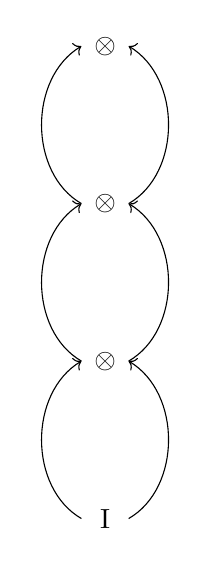
\begin{tikzpicture}[commutative diagrams/every diagram] 
\node (P0) at (2,5) {$\otimes$}; 
\node (P1) at (2,3) {$\otimes$} ; 
\node (P2) at (2,1) {$\otimes$};
\node (P3) at (2,-1) {I};;
\draw [ ->](2.3,-1) to [out = 30, in = -30] (2.3,1); 
\draw [ ->](1.7,-1) to [out = 150, in = -150] (1.7,1); 
\draw [ ->](2.3,1) to [out = 30, in = -30] (2.3,3); 
\draw [ ->](1.7,1) to [out = 150, in = -150] (1.7,3); 
\draw [ ->](2.3,3) to [out = 30, in = -30] (2.3,5); 
\draw [ ->](1.7,3) to [out = 150, in = -150] (1.7,5); 
%\path[commutative diagrams/.cd, every arrow, every label] 
%(P1) edge node[swap] {} (P0)  
%(P1) edge node {} (P0)  
%(P2) edge node[bend left] {} (P1)
%(P3) edge node[swap] {} (P2);
\end{tikzpicture}
\end{center}
\fi

Next we describe some simple ways to construct new circuits from old ones. 
\begin{definition}
(1) The addition/multiplication of two circuits. Take two circuits $G_1$ and $G_2$ with unique output vertices $v_1$ and $v_2$.  Then $G_1 \boxplus G_2$ (resp. $G_1 \boxtimes G_2$) is the circuit that is the union of $G_1$ and $G_2$, plus an extra addition (resp. multiplication) vertex that has $v_1$ and $v_2$ as parents. 
See Figure~\ref{fig: add} for an example. 

(2) The concatenation of two circuits. Let $G_1, G_2$ be two circuits such that the number of output vertices of $G_1$ is equal to the number of inputs of $G_2$. Then we simply ``feed'' the outputs of $G_1$ to inputs of $G_2$. We denote the resulting circuit by 
$G_1 \curvearrowright G_2$. See Figure~\ref{fig: cat} for an example.

(3) The $K$-repeat of a circuit along a subset of vertices. Let $G$ be a circuit and let $S = \{ s_1, \ldots, s_k \}$ be vertices of $G$. 
Let $K$ be a positive integer. Then we keep the vertices $s_i$ and all their ancestors, and copy the rest of the circuit $K$ times. The resulting circuit is denoted by $G^{(K)}_{S}$. See Figure~\ref{fig: repeat} for an example. 

(4) The gluing of two circuits along a subset of vertices. Let $G_1$ and $G_2$ be two circuits and $S_1, S_2$ be subsets of their vertices, such that the subgraph of $G_1$ consisting of ancestors of $S_1$ (including vertices in $S_1$) is isomorphic to the corresponding subgraph in $G_2$. Then the gluing of $G_1$ and $G_2$ along $S_1, S_2$ is the circuit that contains the common subgraph  and the disjoint union of the rest of the two graphs. We denote the new circuit by $G_1 \star_{S_1} G_2$ when $S_2$ and the isomorphism is clear from context. See Figure~\ref{fig: glue} for an example. Note that (3) is a special case of (4). 

\end{definition}

%First
\begin{figure}
\begin{tikzpicture}[commutative diagrams/every diagram] 
\node (P2) at (2,1) {$\otimes$};
\node (P3) at (1,0) {\textbigcircle};;
\node (P4) at (3,-0) {\textbigcircle};;
\path[commutative diagrams/.cd, every arrow, every label] 
(P3) edge (P2)
(P4) edge (P2); 
%\draw [ ->](0.8,-0.8) to (1.8,1); 
%\draw [ ->] (3.2, -0.8) to (2.2,1);
%(P1) edge node[swap] {} (P0)  
%(P1) edge node {} (P0)  
%(P2) edge node[bend left] {} (P1)
%(P3) edge node[swap] {} (P2);
\node (P5) at (2,2) {$G_1$};;
\node (P5) at (7,3) {$G_2$};;
\node (P5) at (12,4) {$G_1 \boxplus G_2$};;


\node (P6) at (5,0) {\textbigcircle};;
\node (P7) at (7,0) {\textbigcircle};;
\node (P8) at (9,0) {\textbigcircle};;
\node (P9) at (6,1) {$\otimes$};
\node (P10) at (8,1) {$\oplus$};
\node (P11) at (7,2) {$\otimes$};
\path[commutative diagrams/.cd, every arrow, every label] 
(P6) edge (P9)
(P7) edge (P9)
(P7) edge (P10)
(P8) edge (P10)
(P9) edge (P11)
(P10) edge (P11);
%\draw [ ->](0.8,-0.8) to (1.8,1); 
%\draw [ ->] (3.2, -0.8) to (2.2,1)
\node (P12) at (11,0) {\textbigcircle
};;
\node (P13) at (10,1) {\textbigcircle};;
\node (P14) at (13,0) {\textbigcircle};;
\node (P15) at (12,1) {\textbigcircle};;
\node (P16) at (15,0) {\textbigcircle};;
\node (P17) at (13,1) {$\otimes$};
\node (P18) at (15,1) {$\oplus$};
\node (P19) at (13,2) {$\otimes$};
\node (P20) at (15,2) {$\otimes$};
\node (P21) at (14,3) {$\oplus$};
\path[commutative diagrams/.cd, every arrow, every label] 
(P12) edge (P17)
(P14) edge (P17)
(P14) edge (P18)
(P16) edge (P18)
(P13) edge (P19)
(P15) edge (P19)
(P17) edge (P20)
(P18) edge (P20)
(P19) edge (P21)
(P20) edge (P21); 
\end{tikzpicture}
\caption{Example of $G_1 \boxplus G_2$}
\label{fig: add}
\end{figure}

% Second example 
\begin{figure}
\begin{tikzpicture}[commutative diagrams/every diagram] 
\node (P1) at (1,0) {\textbigcircle};
\node (P2) at (2,0) {\textbigcircle};;
\node (P3) at (1,1) {$\oplus$};;
\node (P4) at (2,1) {$\otimes$};

\path[commutative diagrams/.cd, every arrow, every label] 
(P1) edge (P3)
(P2) edge (P3)
(P1) edge (P4)
(P2) edge (P4); 

%\draw [ ->](0.8,-0.8) to (1.8,1); 
%\draw [ ->] (3.2, -0.8) to (2.2,1);
%(P1) edge node[swap] {} (P0)  
%(P1) edge node {} (P0)  
%(P2) edge node[bend left] {} (P1)
%(P3) edge node[swap] {} (P2);
\node (P5) at (1.5,2) {$G_1$};;
\node (P5) at (5,2) {$G_2$};;
\node (P5) at (10,3) {$G_1 \curvearrowright G_2$};;
\node (P6) at (5,1) {$\otimes$};
\node (P7) at (4,0) {\textbigcircle};;
\node (P8) at (6,-0) {\textbigcircle};;
\path[commutative diagrams/.cd, every arrow, every label] 
(P7) edge (P6)
(P8) edge (P6); %\draw [ ->](0.8,-0.8) to (1.8,1); 
%\draw [ ->] (3.2, -0.8) to (2.2,1)
\node (P10) at (9,0) {\textbigcircle};
\node (P11) at (11,0) {\textbigcircle};;
\node (P12) at (9,1) {$\oplus$};;
\node (P13) at (11,1) {$\otimes$};
\node (P14) at (10,2) {$\otimes$};
\path[commutative diagrams/.cd, every arrow, every label] 
(P10) edge (P12)
(P11) edge (P12)
(P10) edge (P13)
(P11) edge (P13)
(P12) edge (P14)
(P13) edge (P14); 
\end{tikzpicture}
\caption{Example of $G_1\curvearrowright  G_2$}
\label{fig: cat}
\end{figure}



% Third example 
\begin{figure}
\begin{tikzpicture}[commutative diagrams/every diagram] 

%\draw [ ->](0.8,-0.8) to (1.8,1); 
%\draw [ ->] (3.2, -0.8) to (2.2,1);
%(P1) edge node[swap] {} (P0)  
%(P1) edge node {} (P0)  
%(P2) edge node[bend left] {} (P1)
%(P3) edge node[swap] {} (P2);
\node (P6) at (1,4) {$G$};;
\node (P6) at (10,4) {$G_S^{(2)}$};;

\node (P1) at (0,0) {\textbigcircle};
\node (P2) at (2,0) {\textbigcircle};;
\node (P3) at (0,1) {$\otimes$, $s_1$};;
\node (P4) at (2,1) {$\otimes$, $s_2$};
\node (P5) at (1,2) {$\oplus$};;
\node (P6) at (1,3) {$\otimes$};;
\path[commutative diagrams/.cd, every arrow, every label] 
(P1) edge (P3)
(P2) edge (P3)
(P1) edge (P4)
(P2) edge (P4)
(P3) edge (P5)
(P4) edge (P5)
%(P5) edge (P6)
(P5) edge (P6);
%\draw [ ->](0.8,-0.8) to (1.8,1); 
%\draw [ ->] (3.2, -0.8) to (2.2,1)
\node (P10) at (9,0) {\textbigcircle};
\node (P11) at (11,0) {\textbigcircle};;
\node (P12) at (9,1) {$\otimes$, $s_1$};;
\node (P13) at (11,1) {$\otimes$, $s_2$};
\node (P14) at (9,2) {$\oplus$};
\node (P15) at (11,2) {$\oplus$};
\node (P16) at (9,3) {$\otimes$};
\node (P17) at (11,3) {$\otimes$};
\path[commutative diagrams/.cd, every arrow, every label] 
(P10) edge (P12)
(P11) edge (P12)
(P10) edge (P13)
(P11) edge (P13)
(P12) edge (P14)
(P13) edge (P14)
(P12) edge (P15)
(P13) edge (P15)
(P14) edge (P16)
%(P14) edge[bend right] (P16)
%(P15) edge[bend left] (P17)
(P15) edge (P17);
\end{tikzpicture}
\caption{Example of $G_S^{(K)}$ for $K= 2$ and $S = \{s_1, s_2\}$}
\label{fig: repeat}
\end{figure}



% Final example
\begin{figure}
\begin{tikzpicture}[commutative diagrams/every diagram] 
\node (P1) at (2,2) {$\otimes$};
\node (P2) at (2,1) {$\otimes$ $s_1$};
\node (P3) at (1,0) {\textbigcircle};;
\node (P4) at (3,-0) {\textbigcircle};;
\path[commutative diagrams/.cd, every arrow, every label] 
(P3) edge (P2)
(P4) edge (P2)
(P2) edge (P1)
%(P2) edge[bend right] (P1); 
%\draw [ ->](0.8,-0.8) to (1.8,1); 
%\draw [ ->] (3.2, -0.8) to (2.2,1);
%(P1) edge node[swap] {} (P0)  
%(P1) edge node {} (P0)  
%(P2) edge node[bend left] {} (P1)
%(P3) edge node[swap] {} (P2);
\node (P5) at (2,3) {$G_1$};;
\node (P5) at (7,3) {$G_2$};;
\node (P5) at (13,3) {$G_1 \star_{s_1} G_2$};;


\node (P6) at (5,0) {\textbigcircle};;
\node (P7) at (7,0) {\textbigcircle};;
\node (P8) at (9,0) {\textbigcircle};;
\node (P9) at (6,1) {$\otimes$ $s_2$};
\node (P10) at (8,1) {$\oplus$};
\node (P11) at (7,2) {$\otimes$};
\path[commutative diagrams/.cd, every arrow, every label] 
(P6) edge (P9)
(P7) edge (P9)
(P7) edge (P10)
(P8) edge (P10)
(P9) edge (P11)
(P10) edge (P11);
%\draw [ ->](0.8,-0.8) to (1.8,1); 
%\draw [ ->] (3.2, -0.8) to (2.2,1)
\node (P12) at (11,0) {\textbigcircle};;
\node (P13) at (13,0) {\textbigcircle};;
\node (P14) at (15,0) {\textbigcircle};;
\node (P15) at (12,1) {$\otimes$ };
\node (P16) at (14,1) {$\oplus$};
\node (P17) at (13,2) {$\otimes$};
\node (P18) at (12,2) {$\otimes$};
\path[commutative diagrams/.cd, every arrow, every label] 
(P12) edge (P15)
(P13) edge (P15)
(P13) edge (P16)
(P14) edge (P16)
(P15) edge (P17)
(P16) edge (P17)
%(P15) edge[bend left] (P18)
(P15) edge (P18); 
\end{tikzpicture}
\caption{Example of $G_1 \star_{s_1} G_2$}
\label{fig: glue}
\end{figure}
% End of examples. 




Now we are ready to state our main theorem. Consider a knapsack problem with parameters $v_i (1 \leq i \leq n), w_i (1\leq i\leq n)$ and $W$. 

\iffalse
{\color{red} Hao: one SODA reviewer pointed out a mistake. I think I can fix it by letting 
$M := W + \sum w_i + \sum_i v_i$. Take $T = 2M\log M$, $k_r = 6 M \log M \log(M \log M)$, and $K = 4 \log(M \log M)$. 
In this case, $K$ is still logarithm in the $v_i$ and $W$'s. We can verify that $KT > k_r$, $k_r > T\log T + W' \log W'$. Moreover, we have $Kr_i - k_r \leq 4 \log(M \log M) M \log M - k_r \leq -2 M \log M \log(M\log M) < -M < v_i$, for all $i$. So in the proof we don't have to scale up $K$.}
\fi
\begin{theorem} \label{thm}
There exists a circuit $G = G(v_i, w_i, W)$, and integers $k_m, k_r$ such that 

(1) $G$ has  $O(polylog(v_i, w_i, W) ) \cdot poly(n))$ vertices. 

(2) $k_m, k_r = O( poly(v_i, w_i, W, n))$. 

(3) There exists a set of $n$ vertices $s_1, \ldots, s_n$ in $G$, such that if the length $l_{new}^*(i)$ is the length of $s_i$ in an optimal solution to the relinearize problem on $G$. Then $l_{new}^*(i) (1 \leq i \leq n)$ is an optimal solution to 
\[
\max \sum v_i l_i,  \mbox{ s.t. }  l_i \in \{1, 2\}, \sum w_i l_i \leq W + \sum w_i, 
\]
Hence $l_{new}^*(i) -1 (1 \leq i \leq n)$ is an optimal  solution to the original knapsack problem. 
\end{theorem}
 
  
 
Since our proof is long, we will break it into several parts. First, let $K, T$ be positive integers whose values will be determined later. We  define a circuit 
 \[
 	G^{0}:= \{ ((\cL(w_1) \boxtimes \cL(w_2) ) \cdots \boxtimes \cL(w_n) ) \boxplus \cL(W') ) \curvearrowright \cL(T) \}_S ^{(K)}
 \]
Here $W' = W + \sum_i w_i$, and $S = \{s_1, \ldots, s_n\}$, where $s_i$ is the first non-input vertex in the circuit $\cL(w_i)$. In particular, with no relinearization the length of $s_i$ is equal to 2. Consider the relinearize problem on the circuit $G^0$ and let $l_i$ be the new lengths of $s_i$. Without loss of generality,  we assume that $w_i \leq W$ for all $i$ (if $w_i> W$,  then  any optimal solution of the knapsack problem always have $x_i = 0$, and we can reduce the dimension of the problem by one). 

\begin{lemma} \label{lem: constraint}
Suppose $$k_r > T\log T +W' \log W',$$  and $k_m =1$. Then for any optimal solution to the relinearize problem on $G^0$, the only vertices that could have nonzero relinearization are the $s_i$. 
\end{lemma}

\begin{proof}
We proved that the total cost of evaluating $\cL(T)$ is bounded by $T\log T$, hence relinearizing any single vertex in this circuit has benefit bounded by $T\log T$. The situation is similar for $\cL(W')$. Note that relinearizing verteices in $\cL(W')$ 
could reduce the length of vertices in $\cL(T)$, but the benefit is still bounded above by $T\log T + W'\log W'$. For the same reason, the benefit of relinearizing any vertex in any of the $K$ copies of $\cL(w_i)$ is bounded by $T\log T + w_i \log w_i$. Since $w_i \leq W'$, this completes
the proof.
\end{proof}


\begin{lemma} \label{lem: constraint}
Suppose $KT > k_r$ and $k_m =1$.  Then for any optimal solution to the relinearization problem on $G^0$ we must have 
\[
	\sum l_i w_i \leq  W':= W + \sum_{i =1}^n w_i. 
\]
Here again we recall that $l_i \in \{1, 2 \}$ denote the length of $s_i$ in an optimal solution. 
\end{lemma}



\begin{proof}
Suppose the claim is false. Then there exists $i$ such that $l_i = 2$. We relinearize the vertex $s_i$, which reduces the length of the final output in each  copy of $\cL(w_i)$ by $w_i$, and the length of the output vertex of
$$
(\cL(w_1) \boxtimes \cL(w_2)) \cdots \boxtimes \cL(w_n))$$

is reduced by $w_i$. Since $\sum l_i w_i > W'$, the length of the input vertex in each $\cL(T)$ is reduced by at least one, and the benefit we gain from each $\cL(T)$ is at least $T$. Hence we the benefit 
we collect from relinearizing $s_i$ is at least $KT$, whereas the cost is $k_r$. Since we assumed $KT > k_r$, we know relinearizing the vertex $s_i$ reduces  the total cost. This is a contradiction, since we started with an optimal solution. 
\end{proof}


Now we can starting proving Theorem~\ref{thm}. 




\begin{proof} (of Theorem~\ref{thm}) 
Let 
$M = W + \sum_i w_i + \sum_i v_i$. We start by taking $T = \lceil 5M \log M \rceil$, $k_r = 19 \lceil M \log M \log(M \log M) \rceil$,  $K = 4 \lceil \log(M \log M) \rceil$, and $k_m = 1$. It is easy to see that $K,T, k_r$ are of size polynomial in $W, w_i, v_i$. One can verify that 
$KT > k_r$ and $k_r > T\log T + W' \log W'$. Thus, by Lemma~\ref{lem: constraint}, we have $\sum l_i w_i \leq W'$ if $l_i$ are the new length of $s_i$ in any optimal solution to the relinearization problem on $G^0$. This means we have the correct constraint. However, the costs are wrong: the total cost of evaluating the circuit $G^0$ is given by 
\[
	K(\sum r_i l_i) +\sum_i k_r (2 - l_i) + C, 
\]
where as we proved in Lemma~\ref{lem: one}, $r_i  \leq 4 w_i \log(w_i)$. Here $C$ is the cost of evaluating all the $\cL(T)$ circuits plus all the $\cL(W')$ circuits. The fact that $C$ is a constant follows from Lemma~\ref{lem: constraint}.



Note that the coefficient before $l_i$ is equal to $Kr_i - k_r$, and we want to modify this coefficient to $-v_i$. First, note that 

\begin{align*}
Kr_i - k_r &\leq K 4 w_i \log w_i - k_r  \\
&\leq 4 K \lceil M \log M \rceil - k_r  \\
&\leq -3 \lceil M \log M \log(M\log M) \rceil \\
&\leq -M  \\
&\leq -v_i, \forall i. 
\end{align*}
Let $\lambda_i = k_r - Kr_i - v_i \in \bZ_{\geq 0}$. We claim that there exists a circuit $\cL'(\lambda_i)$ of  such that relinearizing its first non-input vertex  reduces the total multiplication cost by $\lambda_i$. We omit the details of construction of $\cL'$ since it is similar to that of $\cL$. In particular, 
the $\cL'(\lambda_i)$ can be constructed with at most 2 \log (\lambda_i)$ vertices. We then let 
\[
	G^1 = G^0 \star_{s_1} \cL'(\lambda_1), \ldots, 	G^i = G^{i-1} \star_{s_i} \cL'(\lambda_i), \ldots, G^n = G^{n-1} \star_{s_n}  \cL'(\lambda_n)
\]
and set $G = G^n$. Since $\lambda_i < k_r$, we know that in any optimal solution of the relinearize problem on $G$, the vertices in $\cL'(\lambda_i)$ have zero relinearization. Thus, the relinearize problem on $G$ is equivalent to 
\[
\min \sum -v_i l_i + C',  \mbox{ s.t. }  l_i \in \{1, 2\}, \sum w_i l_i \leq W + \sum w_i, 
\]
which is equivalent to 
\[
\max \sum v_i l_i,  \mbox{ s.t. }  l_i \in \{1, 2\}, \sum w_i l_i \leq W + \sum w_i.
\]
This proves part (3) of Theorem~\ref{thm}. Now (1) is clear since the number of vertices in $G$ is bounded by $2K ( \log(T) + \log(W') +  \sum_{i=1}^n \log(w_i) ) + 2\sum_{i=1}^n \log(\lambda_i)$. Hence it is logarithm in the parameters $v_i, w_i, W$ and linear in the number of variables $n$. For (2), note that we set $k_m =1$, so it suffices to prove it for $k_r$. By construction,  $k_r$ is also bounded by a polynomial in $v_i, w_i, W$. This completes the proof.
\end{proof}

\begin{corollary}
The relinearize problem is NP-hard. 
\end{corollary}


\iffalse
\subsection{Further thoughts}
Since the technique of this section can be used to reduce any knapsack problem with multiple constraints
to the Relin problem, we also know that Relin problem has no full polynomial approximation scheme, unless P = NP. But still, does there exist a constant-factor approximation algorithm? For example, does there exist a 1/2-approximation algorithm that runs in polynomial time? 


Answer: probably not? since we can model the set cover problem as a relin problem. 


{\bf Set cover problem}: given $m$ subsets $S_1, \ldots , S_m$  of $[n]$. Find a cover of $[n]$ using the smallest number of subsets. 

It is a theorem that there exists a $c > 0$ such that the set cover problem does not have a $c\ln n$ approximation scheme unless P = NP. In particular, there does not exists a constant-factor approximation scheme, unless P = NP. 

We can reduce the set cover problem to Relin problem. First notice that the input size of the set cover 
problem is $m \times n$. we can enforce the constraints $\sum w_i l_i \leq W$, and since $l_i = (1-x_i)$, 
these turn into $\sum w_i x_i \geq \sum w_i - W$. By choosing the $w_i = 0 or 1$ and $W \leq (m-1)$ carefully, we could enforce the $n$ constraints on $m$ variables, with polynomially many nodes. 

Next we look at the costs: similar to Lemma~3, we now just need $c_{relin} > T\log T + \sum_{k=1}^{n} W_k \log W_k$.  $T$ can be taken to be that $T = n \max \{W_k \log W_k \} \leq mn \log(m)$.   Okay ... so $c_{relin} \leq 2T \log T$. We then choose $K = 2\log T$.  Now total cost should be equal to 
$K(\sum s_i l_i) + \sum c_{relin}(1-l_i) + const$. the coefficient before any $l_i$ is negative, which means that turned to $x_i$ they are positive. Now we just need to add polynomially many branches so that the objective function becomes  $\min \sum x_i$, and we are done! Since we have just added polynomially many nodes, we are sure that the Relin problem has a polynomial size and it models exactly the set cover problem we started with. Okay well....



TODO:maybe it's best to now look at some regular circuits, and see what are the best ways to optimize them using Relinearization. 


\section{Becca's idea of rounding}

The basic idea is: start from the lowest non-input nodes and round up $x$; then at higher nodes, round $x$ up if possible, otherwise round $x$ down
until the new length of the node is at least 2. 

In this way, we always have the rounded lengths are smaller. Meanwhile at each node, the extra relin is at most 1. Hence the total cost of 
this solution is  $$C  \leq C_{opt, LP} + k_r N \leq C_{opt, Int} + k_r N.$$

Can we bound $C_{opt, int}$ from below? Or can we improve the bound? Note the $N$ above is really the cardinality of 
\{node i: $x_i$ is rounded up\}, and we may argue that as long as one $x_i$ is rounded up, we always have a multiplicative node 
as the descendent (grandchild) of $i$. 


\rem{B: I don't think this works, at least not if we allow multiple outputs. If the various nodes in the nested addition have other outputs as well (perhaps more addition?) then it gets confusing. At the very least it needs to be clarified.}





\section{New proof}



Conside a circuit of depth $L$. Denote the level of a node $v$
by $L(v)$. We first define a way to transform an LP solution to another, indexed by each level $l$. For any LP solution $x$, let \[
	V_{+} = \{ v: v \mbox{ is addition node and } x(v) > 0 \}
\]
and 
\[
	V_{+, l }^* = V_{+}^* \cap \{v: L(v) = l\}. 
\]
Then for $1 \leq l \leq L$ we define the $l$-transform as follows. Fix arbitrary $\epsilon \in (0, \min \{x(v) : v \in V_{+, l} \})$. The transform proceeds by level. We start from level $l$,  and reduces the relinearization amount for all nodes in $V_{+, l}$ by $\epsilon$. Then for $k = l+1, \cdots, L$, we fix some arbitary order on the nodes of level $k$ and deal with them one-by-one in the following manner. For a node $v$ of level $k$  if $v$ is an addition node, do nothing; if $v$ is a multiplication node, we increase the relinearization amount of $p_1(v)$ and $p_2(v)$ if necessary, such that the lengths of $p_1(v)$ and $p_2(v)$ are the same as their lengths in the original solution $x$. 





\begin{lemma}
After level $k$ is complete in the $l$-transform, it holds for  every node $v$ of level at most $k$ that: \\
(1) If $v$ is addition, then  $l_{new}(v)  \leq l_{new}^0(v) + \epsilon$. \\
(2) If $v$ is multiplication, then  $l_{new}(w) = l_{new}^0(w)$ for $w = v, p_1(v), p_2(v)$.  
\end{lemma}

\begin{proof}
We prove by induction on $k$. The base case $k = l$ holds by definition. Suppose the claim holds for all levels $\leq k$. Then for a node $v$ of level $k+1$, 

-- if $v$ is addition, then by inductive hypothesis, $l_{new}(w)  \leq l_{new}^0(w) + \epsilon$ for $w = p_1(v), p_2(v)$. Hence $l_{new}(v) \leq l_{new}^0(v) + \epsilon$. This proves (1). 

-- if $v$ is multiplication, then after level $k+1$ in the $l$-transform, we will reduce the lengths of $p_1(v), p_2(v)$ to their original length, and hence reduce the length of $v$ to original, since the relinearization amount of $v$ is not changed after level $k+1$. This proves (2). 
\end{proof}

Let $x'$ denote the solution after the transform. Then it is clear that $x'$ is feasible, given $x$ is feasible. 
Moreover, from (1) in the above lemma, we can deduce that when dealing with each multiplication node in each step, the relinearization amount on each of its parents increase by at most $\epsilon$. Therefore, we have 
\[ 
	\sum_{v} x'(v)  \leq \sum_{v} x(v)  -  |V_{+,l}| \epsilon + 2N_m \epsilon, 
\]
where $N_m$  denotes the number of multiplication nodes in $G$. Also, from (2) we know the multiplication cost of $x'$ is no greater than the multiplication cost of $x$. We can thus deduce the following result.

\begin{theorem}
Suppose the graph $G$ has depth $L$ and $x^*$ is LP-optimal solution to the relinearize problem on $G$. Let $N_{+}^*$ denote the cardinality of the set
\[
V_+^* = \{ v \in G: v \mbox{ is addition node and } x^*(v) > 0 \}
\]
and $N_m$ be the number of multiplication nodes in $G$.  Then 
\[
	N_m \geq \frac{N_+^*}{2L}. 
\]
\end{theorem}




\begin{proof}
Since $V_+^* = \bigcup_{l =0}^{L-1} V_{+,l}^{*}$. It suffices to prove $V_{+,l}^{*} \leq 2N_m$. Now if we take the solution $x^*$ and apply the above transform at level $l$. Then from the above discussion, we arrive at a solution $x'$ with no greater multiplication cost, and 

\[ 
	\sum_v x'(v)  \leq \sum_v x^*(v)  -  |V_{+,l}^*| \epsilon + 2N_m \epsilon, 
\]
Sinec $x^*$ is optimal, we must have $\sum_v x'(v)  \geq \sum_v x^*(v)$, which implies  $V_{+,l}^{*} \leq 2N_m$.
\end{proof}

\begin{corollary}
Becca's rounding algorithm is a $(\frac{2Lk_r}{k_m} +1)$ -approximation to the relinearize problem. 
\end{corollary}
\begin{proof}
Recall that we have $C_{opt} \leq C_{round}  \leq C_{opt} + k_r N_+^*$. The above theorem implies 
that $k_r N_+^*  \leq k_r 2L N_m \leq \frac{k_r}{k_m} 2L k_m N_m \leq \frac{2Lk_r}{k_m}  \cdot C_{opt}$. Hence $C_{round } \leq  (\frac{2Lk_r}{k_m} +1) C_{opt}$.
\end{proof}

\section{Approximation algorithms?}

For example, we will take our graph to be 
[1, None, None, $\otimes$], [2, None, None, $\otimes$], [3, None, None, $\otimes$], [4, (1,2), $\oplus$], [5,(2,3), $\otimes$], [6, (4,5), $\oplus$], [7,(6,6), $\otimes$]. 

Then the LP relaxation problem we have is 

$\min k_m (z_5 + 2l_6)  + k_R(3 - l_1 - l_2 - l_3) + k_R(z_4 - l_4) + k_R(z_5 - l_5) + k_R(z_6 - l_6)$. 

s.t. 
\[
\begin{cases}
l_1 \leq 1 \\
l_2 \leq 1 \\
l_3 \leq 1 \\ 
l_1 \leq z_4 \\
l_2 \leq z_4 \\ 
l_5 \leq l_2 + l_3 \\
l_4 \leq z_4 \\
l_4 \leq z_6 \\
l_5 \leq z_6 \\
l_6 \leq z_6 \\
l_i \geq 0, \qquad \forall i. 
\end{cases}
\]

We can of course write down the dual program. The problem is what it means. 
\fi

\section{An Simple Case}
Assume we are in the situation where each non-input vertex in the circuit has two inputs and at most one output. 
In this case, we have a polynomial time algorithm for the relinearize problem. For a vertex $i$, define $M(i,\ell)$ to be the minimal cost to compute the circuit up to vertex $i$, so that the new length of $i$ is $\ell$.


% Moreover, we have a linear time algorithm that achieves an approximation guarantee of 


Recall that $p_1(i)$ and $p_2(i)$ denote the parents of $i$. If $i$ is a multiplicative vertex, we have 
$$M(i,\ell)=\min_{\ell_1,\ell_2}\{M(p_1(i),\ell_1)+M(p_2(i),\ell_2)+k_r(\ell_1+\ell_2-\ell)+k_m(\ell_1+\ell_2)\}.$$

If $i$ is an addition vertex, we have 
$$M(i,\ell)=\min_{\ell_1,\ell_2}\{M(p_1(i),\ell_1)+M(p_2(i),\ell_2)+k_r(\max\{\ell_1,\ell_2\}-\ell)\}.$$

Here it is important that the vertices all only have a single output, since otherwise $p_1(i)$ and $p_2(i)$ might have a common ancestor, in which case relinearizing this ancestor might benefit both of them.

\begin{claim} Suppose $N  = |V| \ge 2$. Then in the above formulae, it suffices to take the minimum over range $2\le \ell_1, \ell_2 \le N$.
\end{claim}

\begin{proof}
For the input vertices, the lengths is at most $2$. For any non-input vertex $v$, we prove inductively that its length cannot exceed its number of  ancestors. The length is at most $l(p_1(v)) + l(p_2(v))-1$, and by inductive hypothesis, both $l(p_1(v))$ and $l(p_1(v))$ are at most their number of ancestors (or plus one if it happens to be an input vertex). That is, $l(p_1(v)) + l(p_2(v))-1 \le n_1+n_2+1=n$. Here $n_1, n_2, n$ denote the number of ancestors for $p_1(v), p_2(v), v$, respectively. 
\end{proof}

Now our algorithm proceeds as follows. We traverse the $N$ vertices. At each vertex, we compute $M(i,l)$ for $O(N)$ values of $l$, and each computation requires $O(N^2)$ operations. Thus the total running time is $O(N^4)$. Finally, the optimal cost is given by 
$\min_{2 \leq l \leq N} M(v, l)$, where $v$ is the output node of the graph $G$. 
% (Maybe we can improve the analysis with a better bound on the lengths, or maybe we can come up with an algorithm with a better running time.) (Actually $N^4$ could be tight, check this.)
% $\ell_1$ and $\ell_2$ will need to be. It's going to be pretty big - in particular I don't think it needs to be polynomial in the input size to our algorithm. BUT I think it will be polynomial in the lengths themselves, and hence polynomial in the input size that is actually going to be computed with. Would that be a reasonable thing to have happen? Or do we need something a lot more efficient since the whole point of this is to make the computations go faster? Yeah ok, that's way too slow.

% Very simple approximation algorithm: Starting at the input nodes and traversing upward, completely relinearize any node whose child is a multiplication node. This just replaces multiplication work by relinearization work, so the approximation ratio is at most $\frac{k_r}{k_m}$. If this ratio is small, then we get a decent factor approximation.
% Pretty sure this requires nodes only having a single child. Because if a node has two children that are both addition nodes, it is more efficient to relinearize at the parent rather than at both children.

%\begin{fact} Any node whose child is an addition node does not need to be relinearized in an optimal solution.
%\end{fact}

%\begin{fact} At a multiplicative node, we relinearize at most $1$. (If the parents have length greater than $2$, it would be better to relinearize there.)
%\end{fact}

% I think in this simple case it might also be possible to show that a vertex of the linear program is always integral. (Definitely need to check this.)


\section{Conclusion and Future Work}

Fully homomorphic encryption evaluates boolean circuits, and relinearization is a standard technique to reduce the ciphertext sizes after evaluation. In this paper, we consider the goal of optimizing where and how much to perform the relinearization operation in any given circuit, in order to minimize the total computational cost. We formalized it as a discrete optimization problem, and proved that the problem is NP-hard. In the special case where every node has at most one ouptut node, we give a polynomial time algorithm. 

For future directions, it is of interest to design fast approximate algorithms for the relinearization problem. Also, one can aim at optimizing specific circuits that appear in the literature for applications of FHE. Examples include  components of the AES encryption/decryption circuit and machine learning models such as logistic regression or neural network. 

\nocite{*}
\bibliographystyle{alpha}
\bibliography{relinearization}





\end{document}
 